

A Fonte de \textit{Clusters} e Agregados (FoCA), esquematizada na Figura \ref{fig:esquema_foca}, produz nanopartículas metálicas que variam desde $1$ e podem chegar até à $40.000$ átomos (uma partícula de $5nm$ de diâmetro no caso da prata), sendo essa produção por método físico, mais especificamente \textit{sputtering}.

O funcionamento da máquina ocorre basicamente em quatro etapas: primeiramente uma nuvem de átomos é produzida por um \textit{sputtering}; em seguida, são resfriadas por nitrogênio líquido ocorrendo a agregação dos átomos em nanopartículas na presença do gás argônio; na sequência, o feixe de agregados, carregados eletricamente, é guiado por um conjunto de lentes eletrostáticas até chegar no espectrômetro de massa por tempo de voo, onde aproximadamente $10\%$ do feixe é desviado para a análise do espectro de distribuição de massa, sendo possível identificar a massa e, por consequência, o tamanho das partículas produzidas, que será melhor explicado na seção \ref{sec:tof}. Por fim as nanopartículas são depositadas no porta amostras. Na Figura \ref{fig:foto_foca} podemos ver uma foto real da máquina. 

\begin{figure}
  \centering
  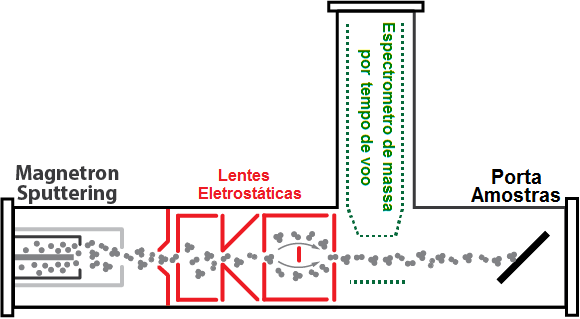
\includegraphics[width=0.8\textwidth]{images/foca/esquematico_foca_pt}
  \caption{ Diagrama da fonte de Fonte de \textit{Clusters} e Agregados. ``\textit{Magnetron Sputtering}'' é a fonte de átomos que se encontra dentro da câmara de agregação. Depois de produzido e agregado, o feixe passa por um conjunto de lentes eletrostáticas. Uma parte do feixe é desviado para o ``\textit{Espectrometro de massa por tempo de voo}'' (ToF), onde é realizada a aquisição do espectro de voo, outra parte é depositada na amostra - Adaptado\cite{livro_vitor}.  }
  \label{fig:esquema_foca}
\end{figure}

\begin{figure}
  \centering
  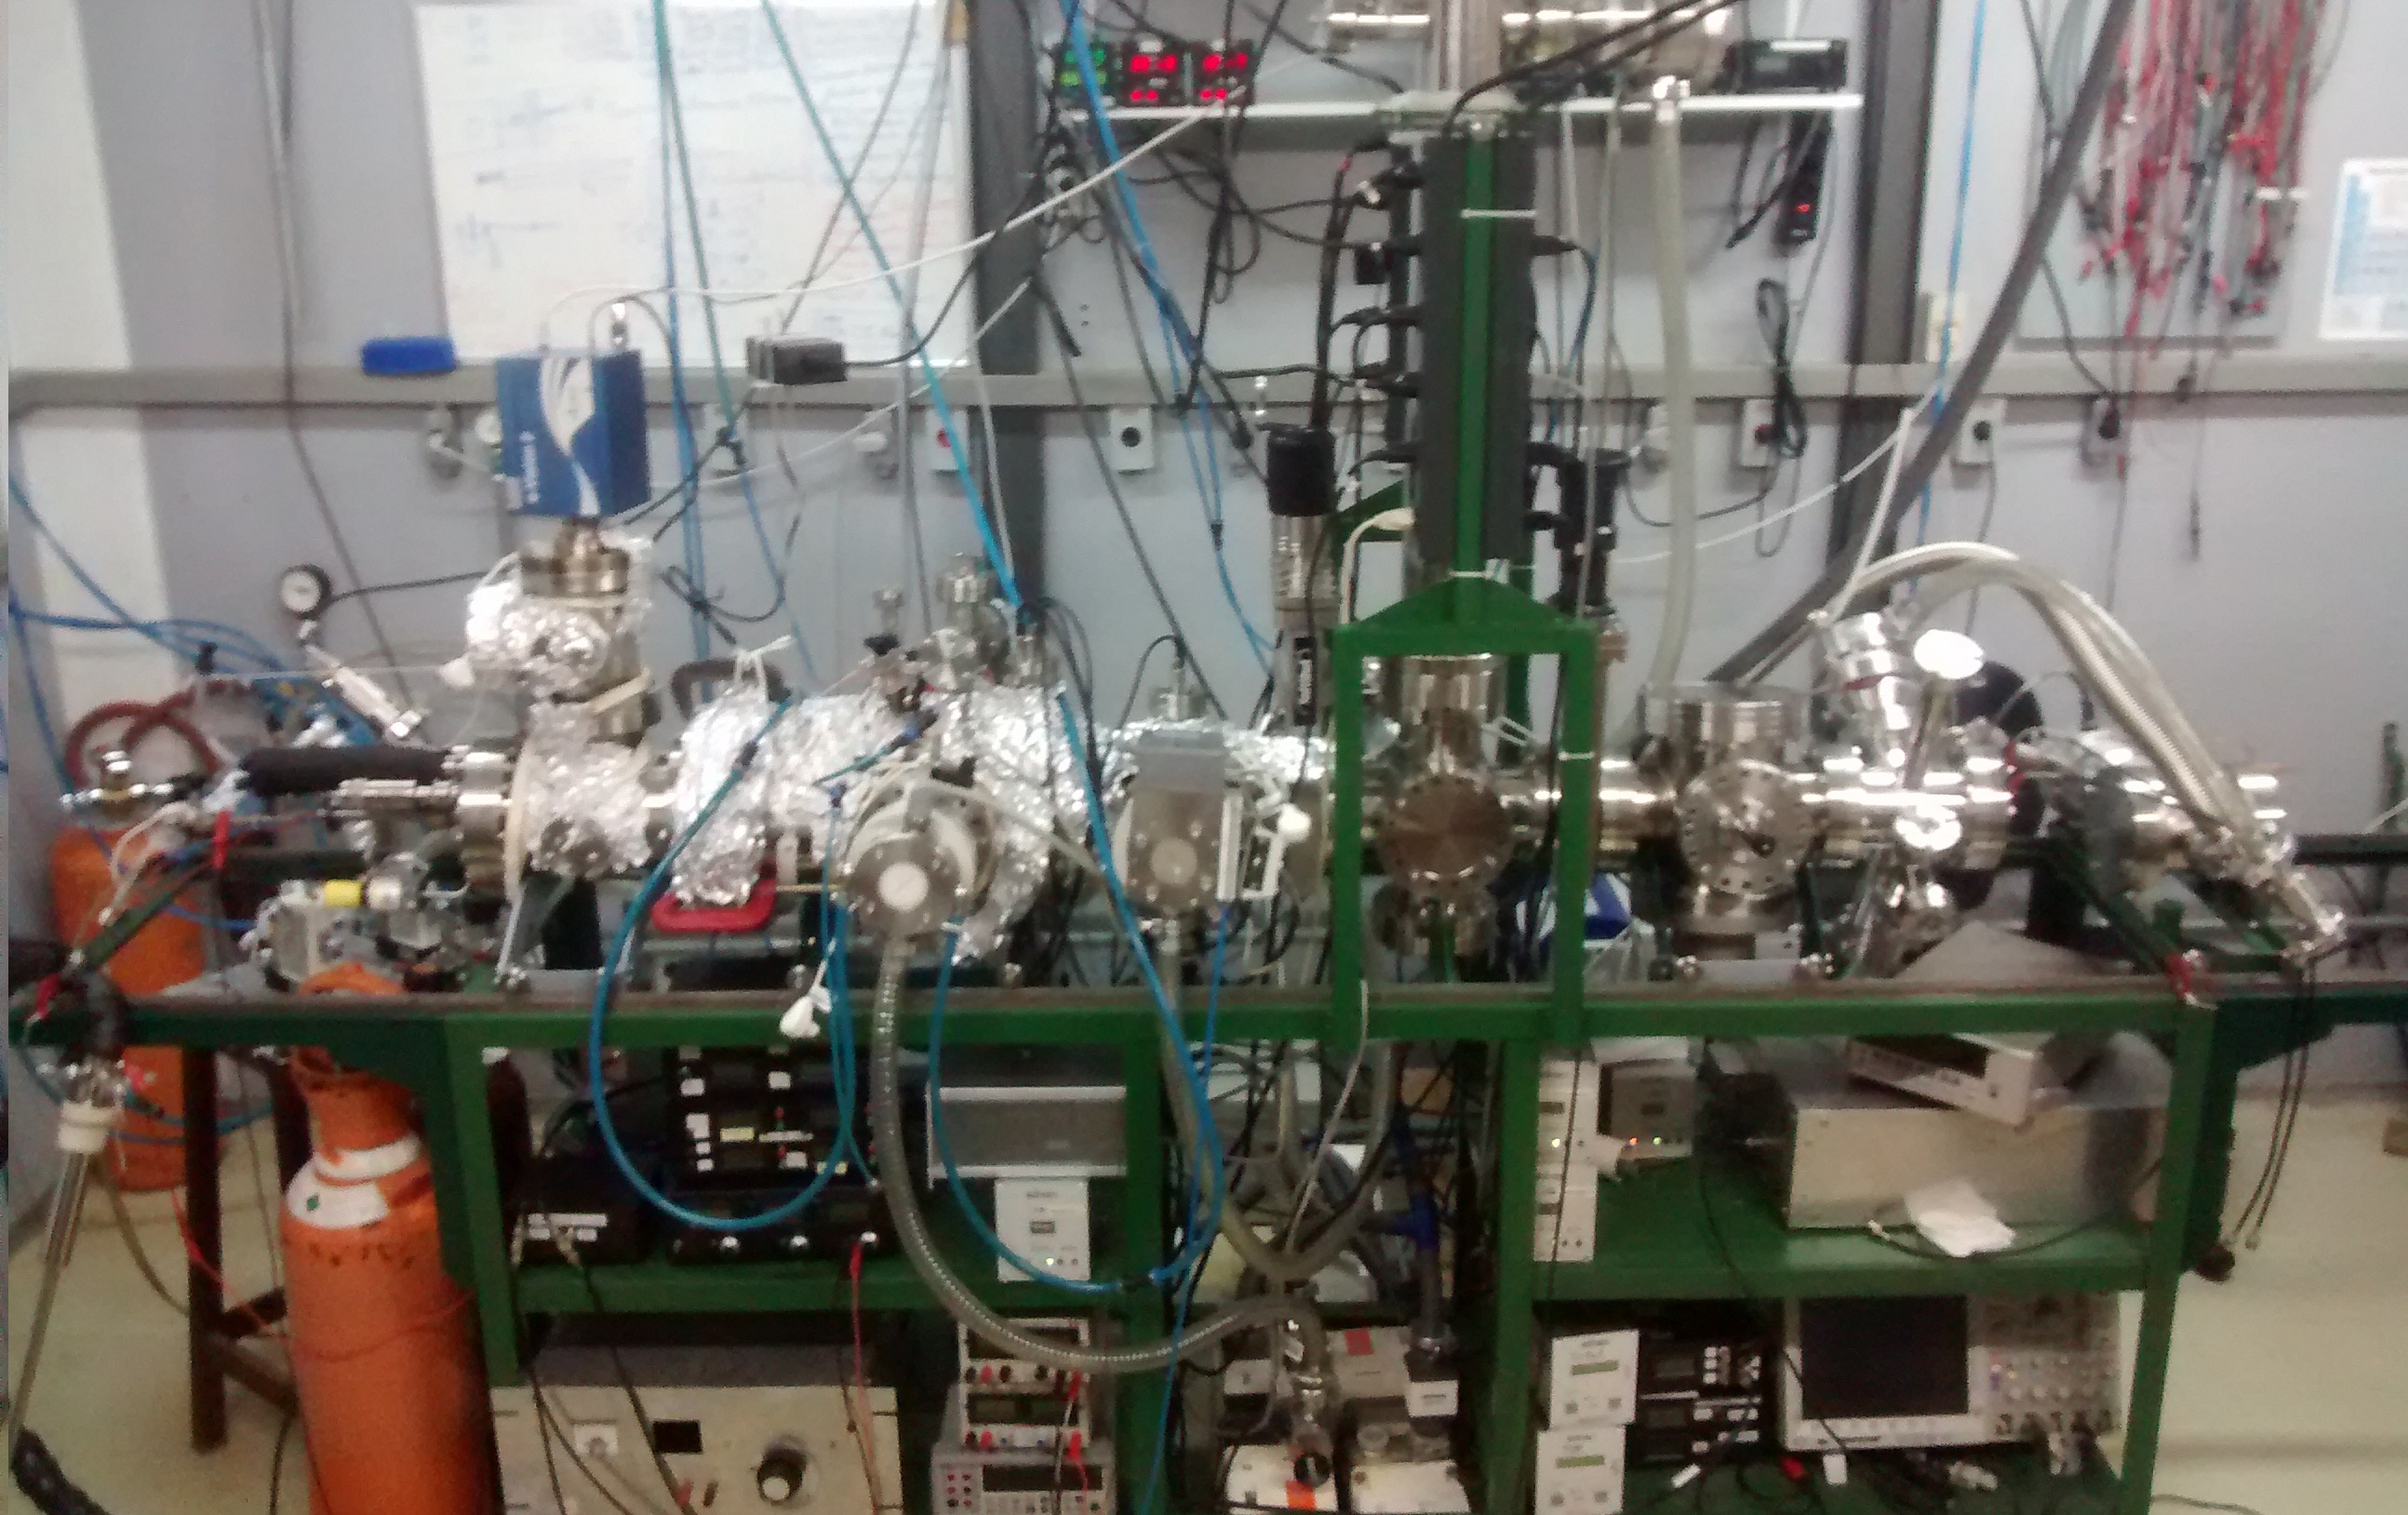
\includegraphics[width=0.7\textwidth]{images/foca/foto_foca}
  \caption{ Imagem real da  Fonte de \textit{Clusters} e Agregados.  }
  \label{fig:foto_foca}
\end{figure}



As lentes eletrostáticas citadas possuem as funções de: focalizar o feixe de íons, retirar as partículas neutras e, de acordo com o potencial aplicado nas lentes podem também funcionar como um filtro em função das energias das partículas. As lentes consistem em uma série de eletrodos de simetria cilíndrica nas quais são aplicadas potenciais. Uma foto das lentes pode ser vista na Figura \ref{fig:foto_lentes}. \textcolor{red}{As palavras skimmer, einzel e bessel não dizem para para o leitor.}

\textcolor{blue}{Com o intuito de colimar e amenizar efeitos de turbulências em grandes na a mistura de gás é utilizado o \textit{Skimmer}. O papel de focalizar o feixe é desenvolvido pelas lentes \textit{Einzel}. As lentes \textit{Bessel-Entrance} e \textit{Bessel-Box} retiram as partículas neutras presentes no feixe e também
atua como filtro de energia para as partículas carregadas.} 

\begin{figure}
  \centering
  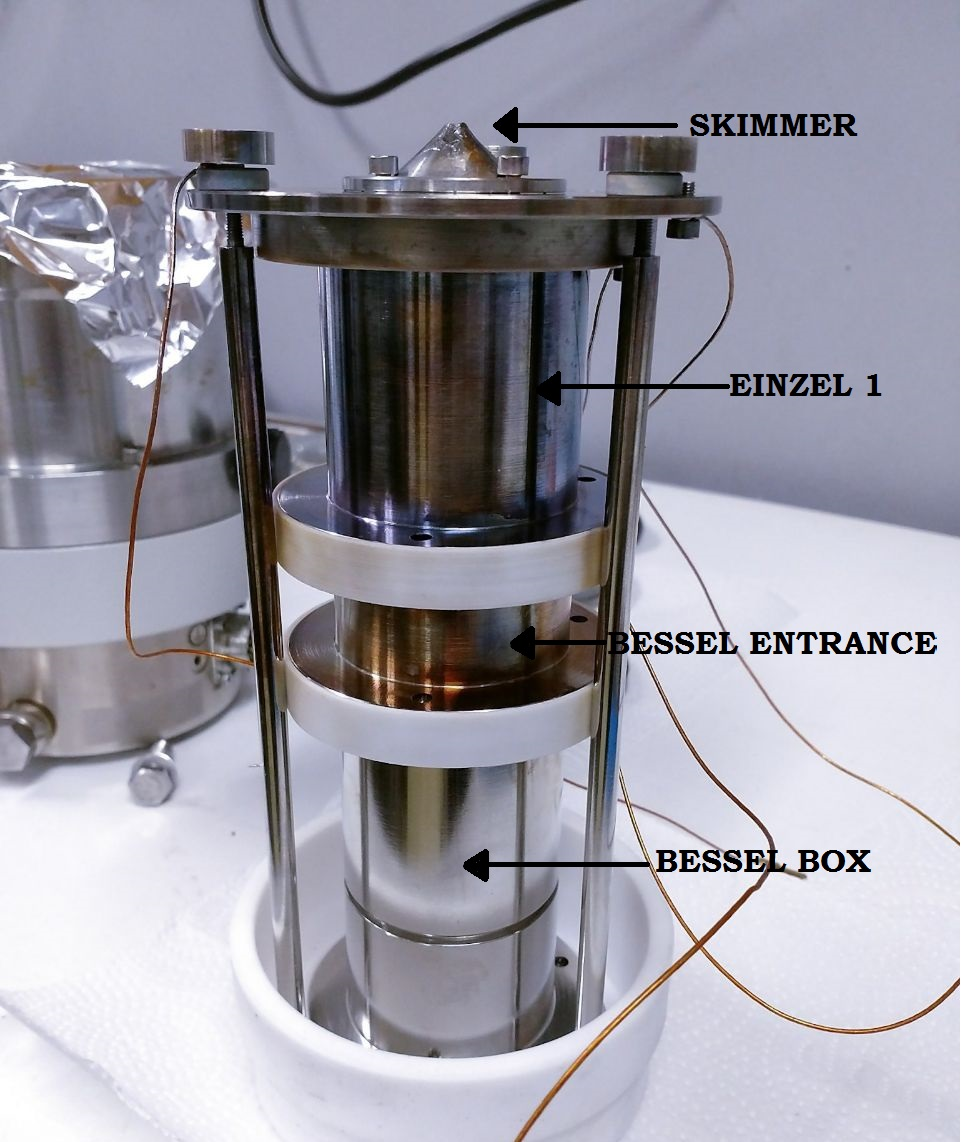
\includegraphics[width=0.6\textwidth]{images/foca/lentes}
  \caption{ Foto da lentes eletrostáticas.  }
  \label{fig:foto_lentes}
\end{figure}


Para gerar a nuvem de átomos, a FoCA utiliza um \textit{magnetron cilíndrico} \cite{ref_artigo_foca}, que caracteriza a produção desses \textit{clusters} por \textit{sputtering}. Aqui o alvo material que dará origem às nanopartículas possui o formato de um fio e fica localizado no eixo do \textit{magnetron}. A versatilidade dessa técnica encontra-se no fato que o alvo é multivalente, podendo ser composto de vários metais, incluindo ligas, como, por exemplo, a mistura ouro e prata, bastando entrelaçar os fios do metal de desejo para isso. Na Figura \ref{fig:magnetron}, podemos ver o plasma gerado no \textit{magnetron cilíndrico}. Pela presença de um campo elétrico, os íons são acelerados em direção ao alvo do metal de interesse e o erodem. Na Figura \ref{fig:alvo} é possível observar um alvo de prata, composto por um único fio, novo e ao lado um já erodido.

\begin{figure}
  \centering
  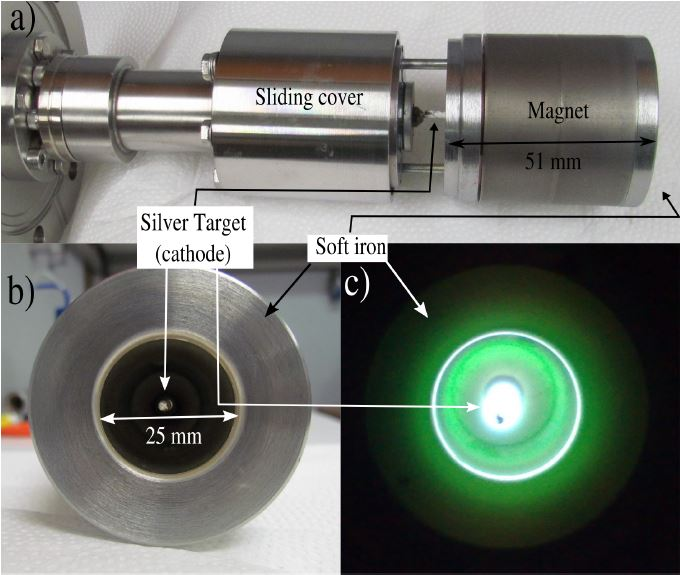
\includegraphics[width=0.75\textwidth]{images/foca/magnetron_cil}
  \caption{ (a) Magnetron cilíndrico oco caseiro com a tampa deslizante retraída para mostrar o alvo de prata. (b) vista frontal. (c) Vista frontal com plasma aberto. Observe a cor esverdeada ao redor do alvo, tipicamente vista na formação de plasma prateado.\cite{livro_vitor} }
  \label{fig:magnetron}  
\end{figure}



\begin{figure}
  \centering
  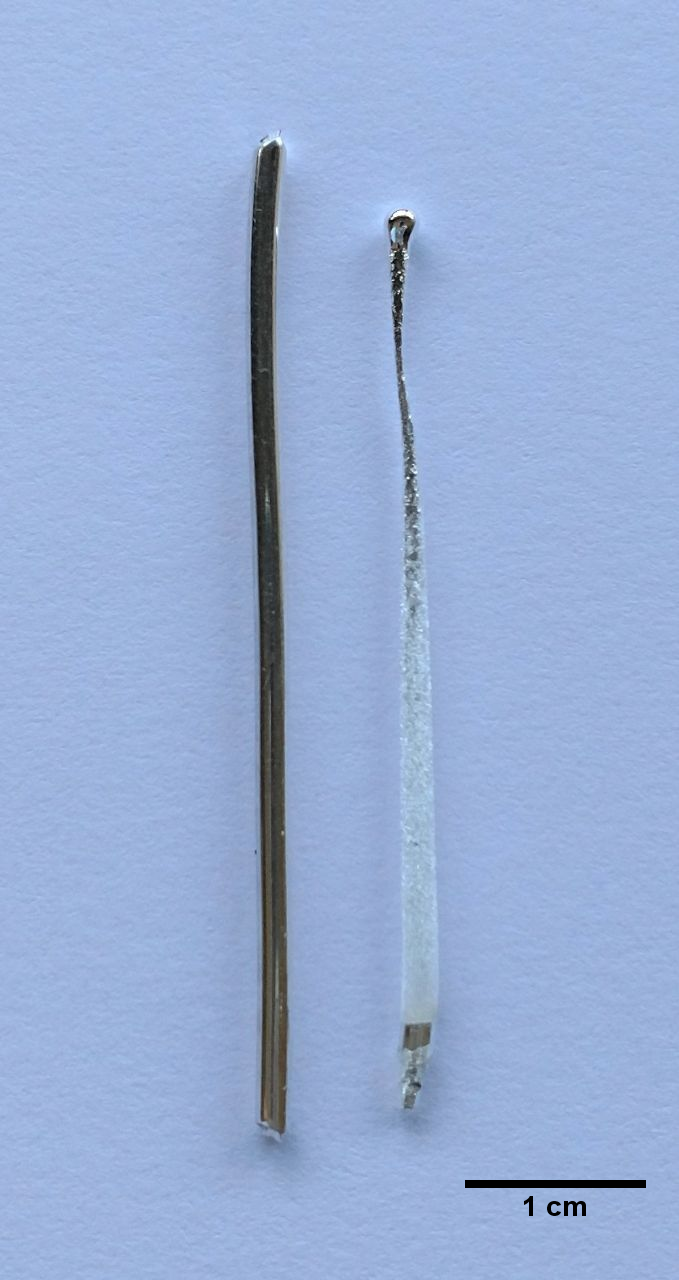
\includegraphics[width=0.3\textwidth]{images/foca/alvo}
  \caption{ Foto de um alvo de prata de fio único. À esquerda temos um alvo novo e à direita temos um alvo já corroído.  }
  \label{fig:alvo}
\end{figure}
